\documentclass{beamer}
\usetheme{Szeged}
%\usetheme{Copenhagen}
\usecolortheme{beaver}

\usepackage[utf8]{inputenc}

\usepackage{listings, float, graphicx, lipsum, parallel, verbatim, mathtools, amssymb, hyperref}

\title{EmotionRecognition}
\author{Edoardo De Matteis}

\institute[Sapienza Università di Roma Computer Science]

\begin{document}

\frame{\titlepage}

\begin{frame}
    \frametitle{Goal}
    The goal is to develop a \textbf{facial emotion recognition} system able to determine if a face exspresses a positive or negative emotion.
    note that emotions are something deeper than just facial expressions.
\end{frame}

\begin{frame}
    \frametitle{Use cases of facial recognition}
    \begin{itemize}
        \item Mood analysis.
        \item Prevention of terrorist attacks.
        \item Refinement of marketing strategies.
        \item Behavioral analysis.
    \end{itemize}
\end{frame}

\begin{frame}
    \frametitle{Strategy}
    The strategy follows this pipeline:
    \begin{enumerate}
        \item Face detection with haar cascade classifiers.
        \item Feature extraction with landmark features.
        \item Classification with support vector machines.
    \end{enumerate}
    Note that to get good results is reccomended to use neural networks.
\end{frame}

\begin{frame}
    \frametitle{Dataset}
    The adopted dataset is \textit{First Affect-in-the-Wild} (affwild), it is composed of videos and to each frame is associated an emotion. 
    Emotions are represnted as points on a 2D cartesian plane.
\end{frame}

\begin{frame}
    \frametitle{Emotion representation}
    \begin{figure}
        \centering
        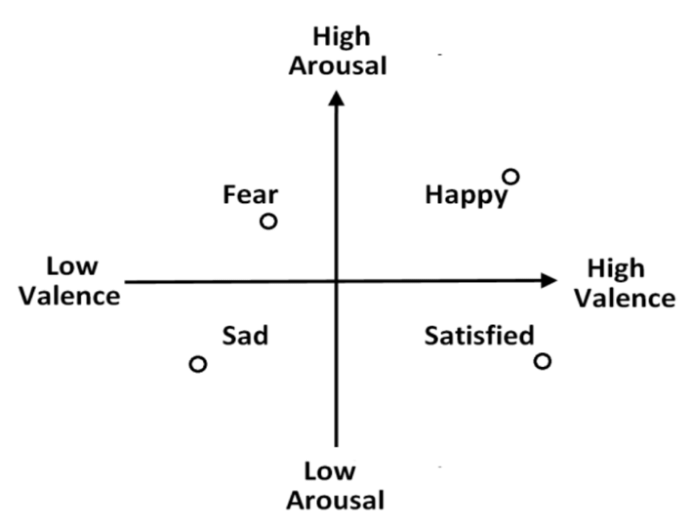
\includegraphics[scale=0.3]{../paper/images/emotion-classification.png}
    \end{figure}
\end{frame}

\begin{frame}
    \frametitle{Design choices}
    The system is written in the \textit{Python} language and uses \textit{OpenCV}.
    The main design choices regard:
    \begin{itemize}
        \item How to encode the sample set.
        \item How to deal with responses.
        \item Choose the SVM.
        \item Online demo.
    \end{itemize}
\end{frame}

\begin{frame}
    \frametitle{Samples}
    \begin{itemize}
        \item To represent expressions I considered only landmark points corresponding to eyes and mouth.
        Instead of a vector of points we have a 1D vector of coordinate points.
        
        \item I assume that the face we're interested in is the foreground one. For this reason I pick the one with the maximum euclidean distance between te first and last point.
    \end{itemize}
\end{frame}

\begin{frame}
    \frametitle{Feature extraction}
    \begin{center}
        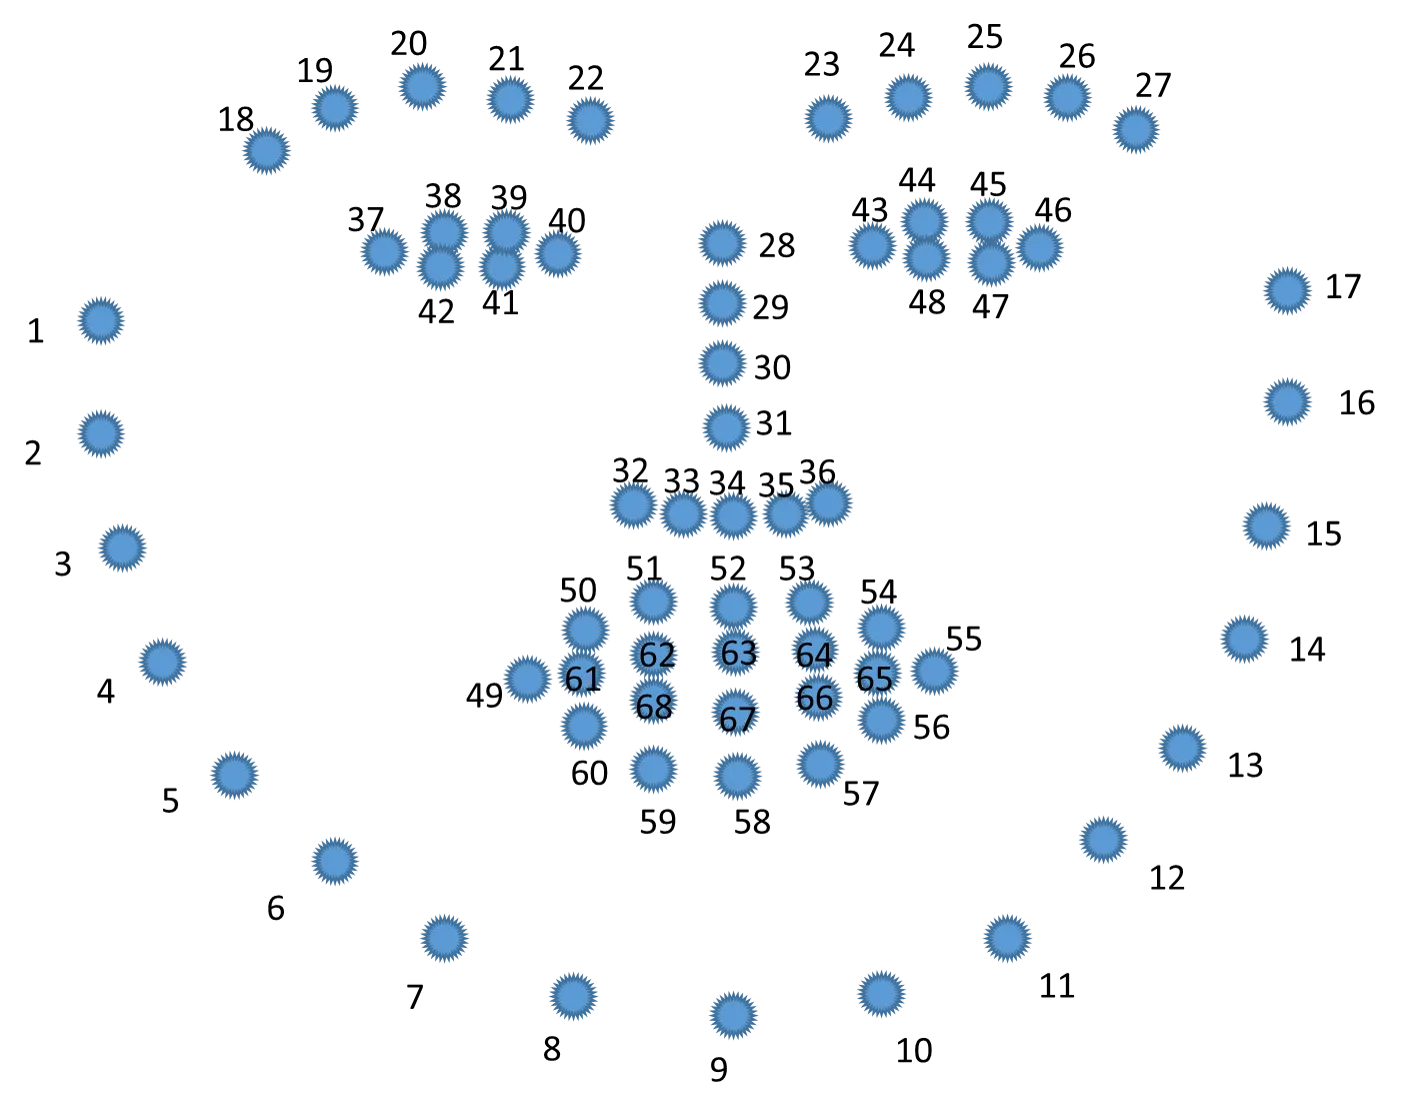
\includegraphics[scale=0.15]{../paper/images/landmark.png}
    \end{center}
\end{frame}

\begin{frame}
    \frametitle{Feature extraction}
    \begin{center}
        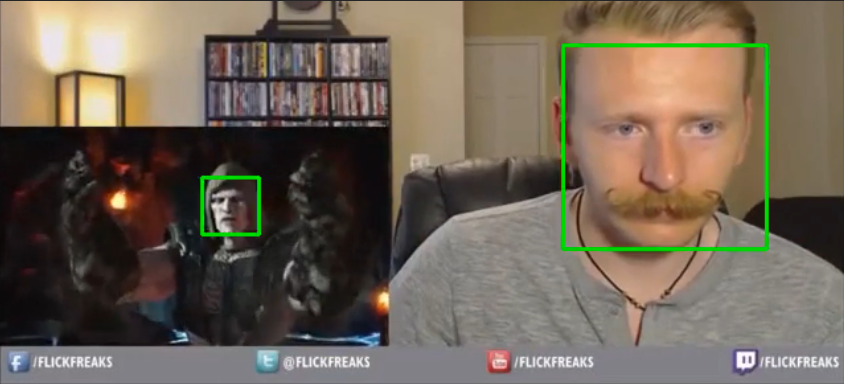
\includegraphics[scale=0.3]{../paper/images/309mp4_double_face.png}
    \end{center}
\end{frame}

\begin{frame}
    \frametitle{Responses}
    Since classifying between too many classes could lower performances I decided I decided to drop arousal and just consider valence, thus not classifying emotions but only positive and negative ones.

    For each frame were considered only valences $v$ such that $ -0.5 < v < 0.5$, in the end were extracted 136909 examples. 
\end{frame}

\begin{frame}
    \frametitle{SVM classifier}
    The \textit{OpenCV} SVM classifier has terrible performances, for this reason is used the better one \textit{scikit-learn}, it uses a RBF kernel.
    Still the \textit{OpenCV} SVM with RBF is worse than the \textit{scikit-learn} one.

    \begin{equation}
        K(x,x') = \exp \left(\frac{||x-x'||^2}{2\sigma^2}\right)
    \end{equation}
\end{frame}

\begin{frame}
    \frametitle{Online demo}
    I noticed how given the same frame landmark points are more easily found than bounding boxes with haar cascades. 
    To make the demo smoother I first detect bounding boxes and then landmark features.
\end{frame}

\begin{frame}
    \frametitle{Performance evaluation}

    \begin{table}[h!t]
        \centering
        \caption{Scores for the classifiers with a RBF kernel.}
        \label{tab:scores}
        \begin{tabular}{lcc}
            & scikit-learn & OpenCV \\
            Accuracy & 0.805 & 0.491 \\
            Precision & 0.814 & 0.421 \\
            Recall & 0.639 & 0.860 \\
            F1 & 0.358 & 0.283 \\
        \end{tabular}
    \end{table}

    \begin{itemize}
        \item Receiver Operator Characteristic curve.
        \item Detection Error Tradeoff curve.
        \item Equal Error Tradeoff.
    \end{itemize}

\end{frame}

\begin{frame}
    \frametitle{ROC curve}
    \begin{center}
        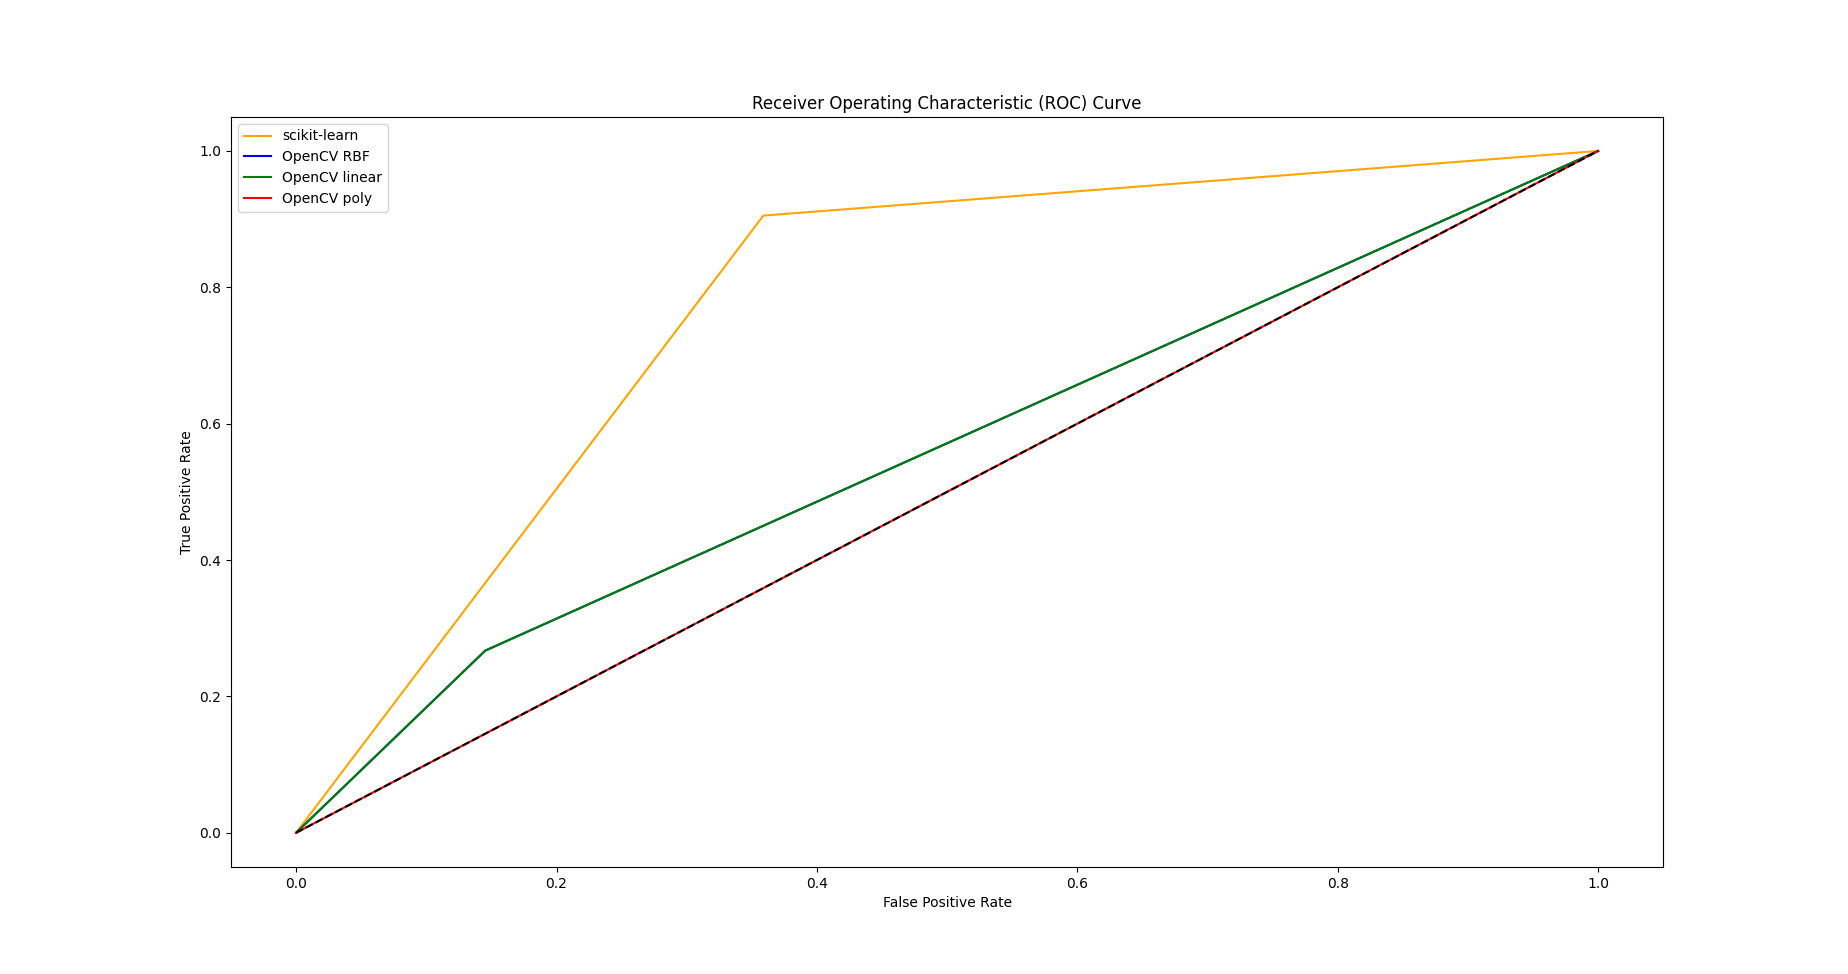
\includegraphics[scale=0.23]{../paper/images/roc.png}
    \end{center}
\end{frame}

\begin{frame}
    \frametitle{Detectior Error Tradeoff curve}
    \begin{center}
        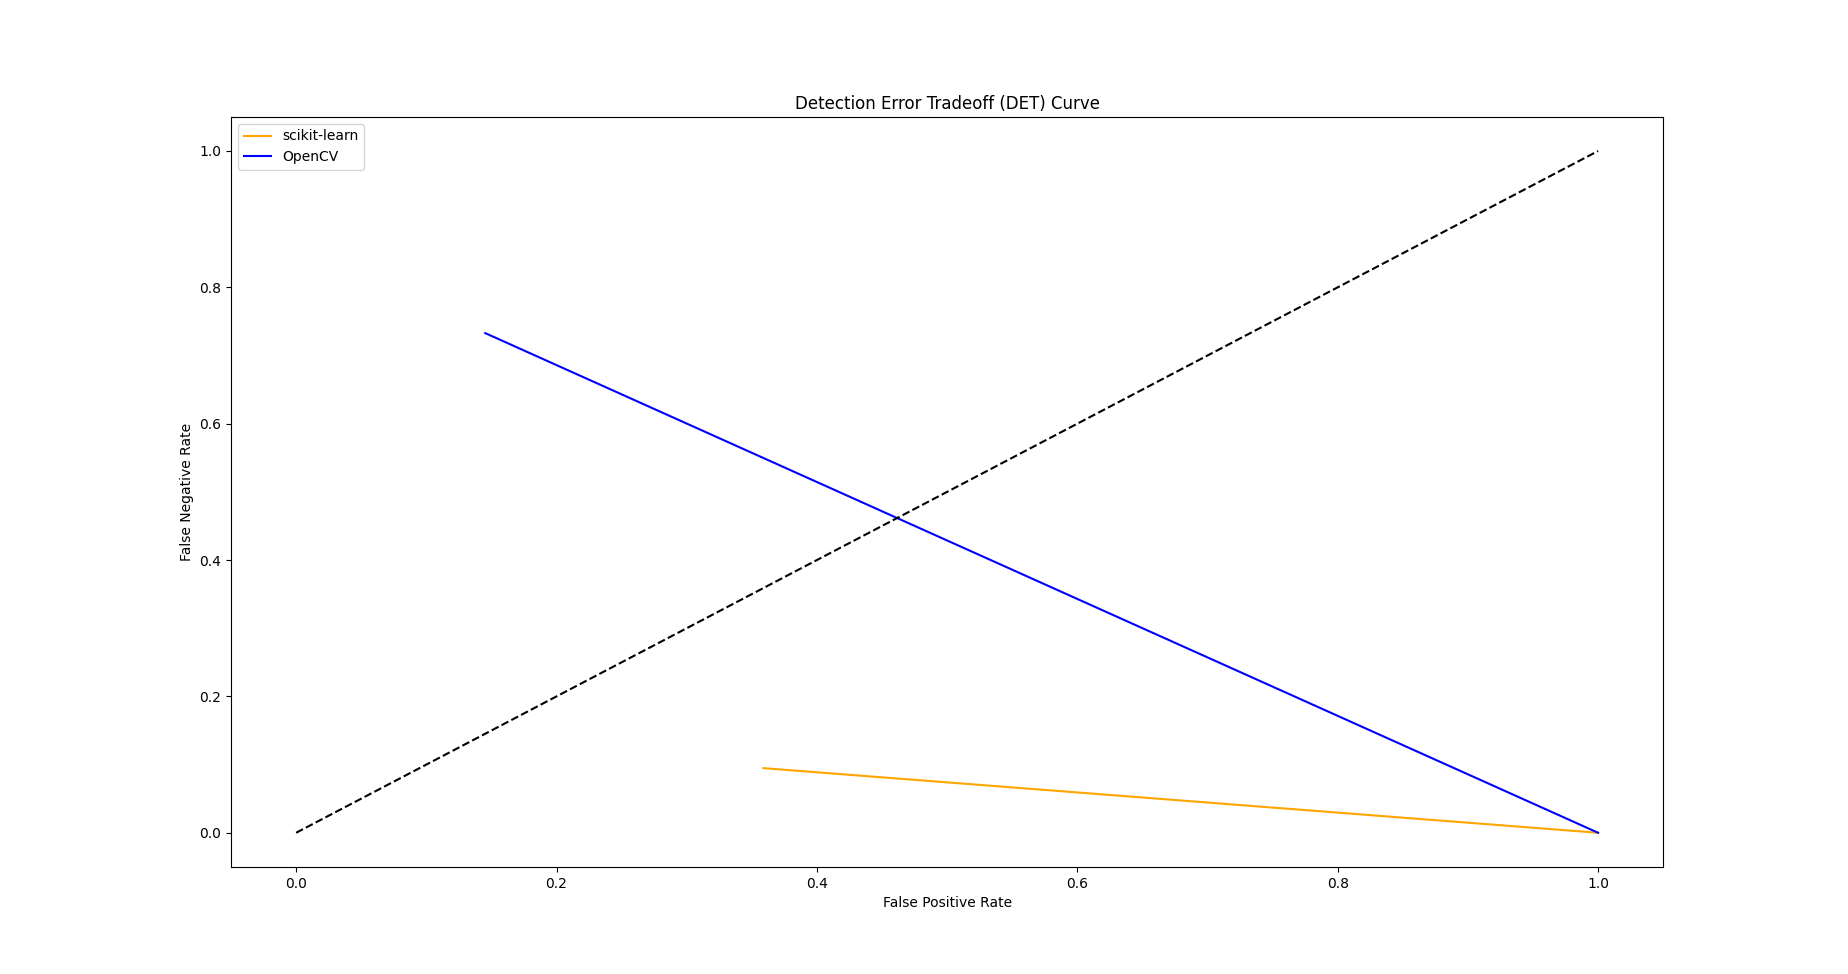
\includegraphics[scale=0.23]{../paper/images/det.png}
    \end{center}
\end{frame}

\begin{frame}
    \frametitle{Equal Error Tradeoff}
    \begin{center}
        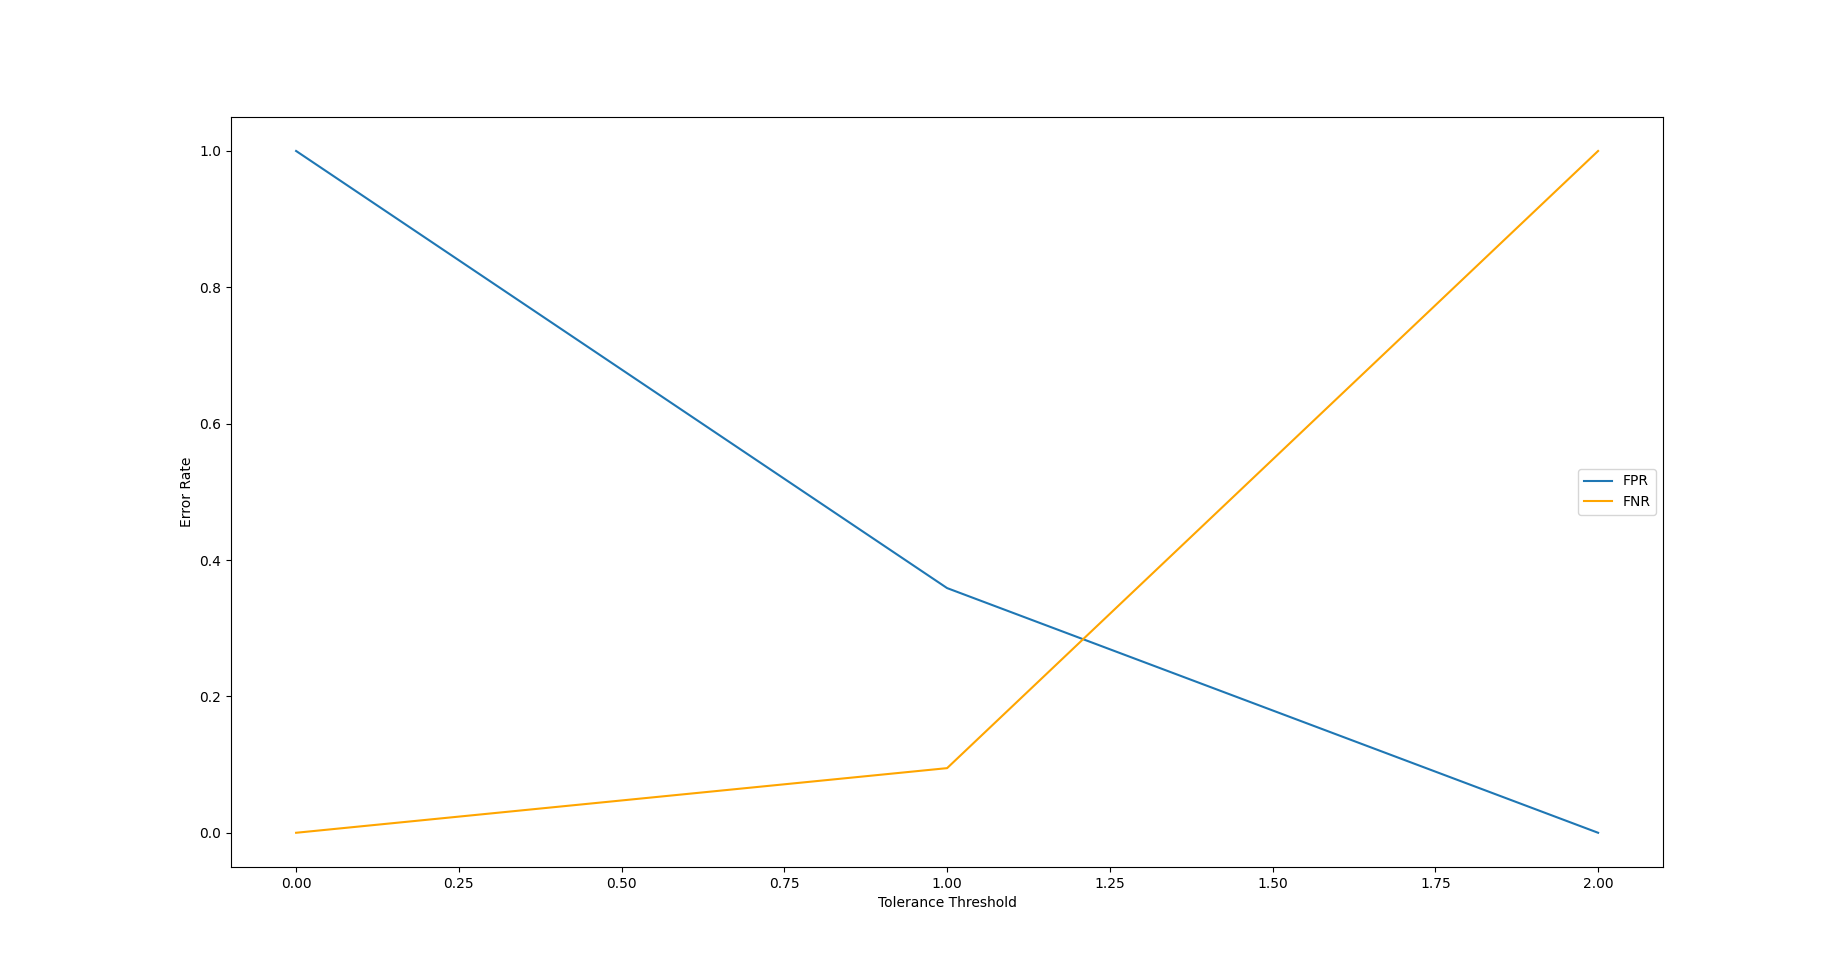
\includegraphics[scale=0.23]{../paper/images/eet.png}
    \end{center}
\end{frame}

\begin{frame}
    \frametitle{Conclusions}
    \begin{itemize}
    \item The scikit-learn SVM classifier has quite good results, with a 76\% AUC.
    \item The polynomial kernel performs worse than the linear, it seems due to overfitting.
    \item In the online demo PIE variations are crucial for the outcome.
    \end{itemize}
\end{frame}

\begin{frame}
    \frametitle{Future works}
    \begin{itemize}
        \item Predict both valence and arousal.
        \item Use a neural network instead of a SVM.
    \end{itemize}
\end{frame}

\begin{frame}
    \begin{center}
        \Large{\textit{Thank you.}}        
    \end{center}
\end{frame}

\end{document}
